\documentclass[10pt,a4paper]{article}
\usepackage[margin=0.8in]{geometry}
\usepackage[T1]{fontenc}
\usepackage[utf8]{inputenc}
\usepackage{lmodern}
\usepackage{microtype}
\usepackage{xcolor}
\usepackage{hyperref}
\usepackage{booktabs}
\usepackage{enumitem}
\usepackage{listings}
\usepackage{tikz}
\usetikzlibrary{arrows.meta,positioning,shapes.geometric}

\hypersetup{
  colorlinks=true,
  linkcolor=blue!40!black,
  urlcolor=blue!40!black,
  citecolor=blue!40!black
}

\lstdefinestyle{code}{
  basicstyle=\ttfamily\small,
  breaklines=true,
  columns=fullflexible,
  frame=single,
  keepspaces=true,
  showstringspaces=false,
  tabsize=2
}
\lstset{style=code}

\title{\textbf{Forml Compiler: Technical Reference \& Architecture Manual}}
\author{Compiler Pipeline Documentation}
\date{\today}

\begin{document}
\maketitle

\section{Introduction \& Pipeline Workflow}
The Forml Compiler is a lightweight, hand-written C++17 front-end pipeline for the Forml Domain-Specific Language (DSL). It compiles Forml source code into a standardized JSON Abstract Syntax Tree (AST) suitable for form rendering engines and frontend integrations.

The compilation process is coordinated by the public entry point \texttt{forml::compileForml()} inside \texttt{forml\_bridge.cpp} and proceeds sequentially:

\begin{enumerate}[leftmargin=*]
  \item \textbf{Lexical Analysis (Lexing):} The input string is tokenized into a stream of \texttt{Token} objects by the \texttt{Lexer}. Syntax/character-level errors are collected without throwing exceptions.
  \item \textbf{Syntactic Analysis (Parsing):} A recursive-descent parser consumes the tokens, enforcing Forml's EBNF grammar. It constructs a strongly typed AST rooted at \texttt{FormNode}. If syntax errors occur, the parser runs panic-mode recovery to continue parsing.
  \item \textbf{Semantic Analysis (Validation):} The \texttt{SemanticAnalyzer} performs symbol validation, check-referencing variables, groups, validation rule types, and checking for duplicate definitions.
  \item \textbf{AST Serialization:} The visitor-pattern-based \texttt{JsonSerializer} traverses the AST, compiling it into a JSON format.
  \item \textbf{Bridge Output Packaging:} The final result is returned as a JSON string containing \texttt{"success"} (boolean), \texttt{"ast"} (JSON payload or null), and \texttt{"diagnostics"} (list of lexical, parse, and semantic issues).
\end{enumerate}

\begin{center}
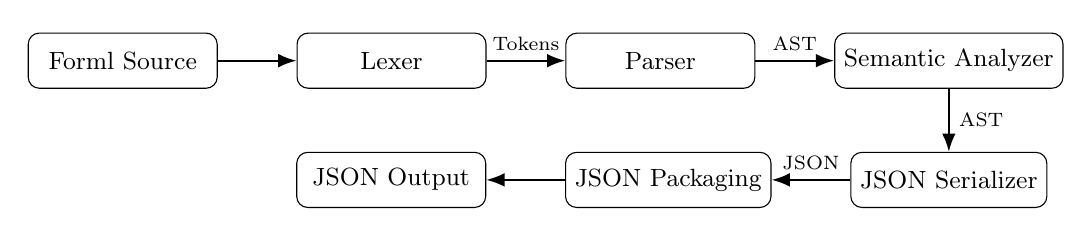
\begin{tikzpicture}[
  node distance=0.8cm and 1cm,
  box/.style={draw, rectangle, align=center, minimum width=2.4cm, minimum height=0.7cm, font=\small, rounded corners},
  arr/.style={-Latex, thick}
]
  \node[box] (src) {Forml Source};
  \node[box, right=of src] (lex) {Lexer};
  \node[box, right=of lex] (par) {Parser};
  \node[box, right=of par] (sem) {Semantic Analyzer};
  \node[box, below=of sem] (ser) {JSON Serializer};
  \node[box, left=of ser] (pack) {JSON Packaging};
  \node[box, left=of pack] (out) {JSON Output};
  
  \draw[arr] (src) -- (lex);
  \draw[arr] (lex) -- node[above, font=\scriptsize] {Tokens} (par);
  \draw[arr] (par) -- node[above, font=\scriptsize] {AST} (sem);
  \draw[arr] (sem) -- node[right, font=\scriptsize] {AST} (ser);
  \draw[arr] (ser) -- node[above, font=\scriptsize] {JSON} (pack);
  \draw[arr] (pack) -- (out);
\end{tikzpicture}
\end{center}

\section{Component \& File Directory}
The codebase is cleanly separated into interface declarations (\texttt{include/forml/}) and source implementations (\texttt{src/}):

\begin{table}[h!]
\centering
\small
\begin{tabular}{llp{7.5cm}}
\toprule
\textbf{Header File} & \textbf{Source File} & \textbf{Component Role \& Primary Responsibility} \\
\midrule
\texttt{token.hpp} & \texttt{token.cpp} & Defines \texttt{TokenType} enum, token structure, and stringifier utilities. \\
\texttt{diagnostics.hpp} & \texttt{diagnostics.cpp} & Non-throwing diagnostics aggregator (\texttt{DiagnosticEngine}) for warnings/errors. \\
\texttt{lexer.hpp} & \texttt{lexer.cpp} & Main character-by-character scanner; handles keywords, literals, and comments. \\
\texttt{ast.hpp} & \texttt{ast.cpp} & AST tree nodes using \texttt{unique\_ptr} exclusive-ownership. \\
\texttt{ast\_visitor.hpp} & --- & Abstract interface for AST double-dispatch visitor operations. \\
\texttt{parser.hpp} & \texttt{parser.cpp} & Hand-written recursive-descent parser; implements EBNF rules. \\
\texttt{semantic\_analyzer.hpp} & \texttt{semantic\_analyzer.cpp} & Symbol resolution, type checks, duplicate declarations, and validation checks. \\
\texttt{json\_serializer.hpp} & \texttt{json\_serializer.cpp} & AST walker that translates AST structures into JSON AST schema. \\
\texttt{forml\_bridge.hpp} & \texttt{forml\_bridge.cpp} & High-level C++ pipeline orchestrator; packs result JSON with diagnostics. \\
\bottomrule
\end{tabular}
\end{table}

\section{Compiler Phase Implementation Details}

\subsection{Lexer (Lexical Scanning)}
The \texttt{Lexer} translates source text character-by-character. It tracks line and column offsets to support accurate error diagnostics.
\begin{itemize}[leftmargin=*]
  \item \textbf{Maximal Munch:} Distinguishes operators with common prefixes (e.g. \texttt{==} vs \texttt{=}, \texttt{!=} vs \texttt{!}, \texttt{\&\&} vs \texttt{\&}).
  \item \textbf{Identifiers/Keywords:} Matches alphabetical lexemes, verifying if they correspond to reserved keywords (e.g., \texttt{form}, \texttt{field}, \texttt{var}) or are standard identifiers.
  \item \textbf{Literals:} Extracts double-quoted strings (handling unterminated errors) and decimal/integer numbers.
\end{itemize}

\subsection{Parser (Syntactic Analysis)}
The parser enforces the syntactic structure outlined in \texttt{EBNF\_grammar.md} through mutually recursive functions corresponding to grammar production rules (e.g., \texttt{parseField()}, \texttt{parseCondition()}).
\begin{itemize}[leftmargin=*]
  \item \textbf{Precedence Climbing:} Handled directly through the call chain hierarchy to enforce correct binary operator binding precedence:
    \begin{itemize}
      \item \textit{Logic operators:} \texttt{||} (lowest, \texttt{parseCondition()}) $\rightarrow$ \texttt{\&\&} (\texttt{parseLogicTerm()}) $\rightarrow$ comparisons (\texttt{parseLogicFactor()}).
      \item \textit{Math operators:} \texttt{+} and \texttt{-} (\texttt{parseExpression()}) $\rightarrow$ \texttt{*} and \texttt{/} (\texttt{parseMathTerm()}) $\rightarrow$ factors (\texttt{parseMathFactor()}).
    \end{itemize}
  \item \textbf{Error Recovery:} Implements panic-mode recovery. When mismatched tokens are encountered via \texttt{expect()}, the engine registers a diagnostic and syncs to a safe boundary (statement starters like \texttt{field}, \texttt{page}, or block closers \texttt{\}}).
\end{itemize}

\subsection{Semantic Analyzer (Validation checks)}
Once the AST is built, the compiler walks the tree to check semantic validity before serialization:
\begin{itemize}[leftmargin=*]
  \item \textbf{Scope checks:} Collects all declared page names, variables, groups, and field names globally at the form level. Reports duplicates.
  \item \textbf{Reference checks:} Resolves names referenced in conditions, math compute statements, and \texttt{repeat count} expressions to guarantee they map to defined fields or variables.
  \item \textbf{Type compatibility:} Restricts validation parameters (e.g., checking that \texttt{min}/\texttt{max} bounds are only specified for numeric fields and \texttt{minLength}/\texttt{maxLength}/\texttt{pattern} are only specified for text/email fields).
  \item \textbf{Constants validation:} Validates that \texttt{var} statements are assigned literal values, not dynamic expressions or identifier references.
\end{itemize}

\subsection{JSON AST Serializer}
The \texttt{JsonSerializer} implements the \texttt{ASTVisitor} interface. It performs a type-safe traversal of all AST nodes. It formats nodes into structured JSON objects following the schema in \texttt{JSON\_SCHEMA.md}. For reentrancy safety, visitors build nodes locally and push them up the call stack rather than mutating shared class variables.

\section{JSON AST Structure Example}
Below is a sample of the JSON AST structure generated by compiling a simple form:
\begin{lstlisting}
{
  "success": true,
  "diagnostics": [],
  "ast": {
    "type": "Form",
    "name": "Customer Feedback",
    "varDeclarations": [
      {
        "type": "VarDeclaration",
        "name": "base",
        "value": {
          "type": "Value",
          "valueKind": "number",
          "numberValue": 2.0
        }
      }
    ],
    "pages": [
      {
        "type": "Page",
        "name": "Main",
        "statements": [
          {
            "type": "Field",
            "name": "age",
            "fieldType": "integer",
            "validation": {
              "type": "ValidationBlock",
              "min": 0.0,
              "max": 120.0
            }
          }
        ]
      }
    ]
  }
}
\end{lstlisting}

\end{document}
